

\chapter{Simulation of a Memristor as a Coupled Electronic Device} % Main chapter title

\label{Chapter4} % Change X to a consecutive number; for referencing this chapter elsewhere, use \ref{ChapterX}

\lhead{Chapter 4. \emph{Simulation of a Memristor as a Coupled Electronic Device}} % Change X to a consecutive number; this is for the header on each page - perhaps a shortened title
\begin{doublespace}

An organic memristor which is an example of a coupled ionic/electronic device is simulated in this thesis. The memristor uses a strip of PEDOT:PSS as a conductor. A drop of an electrolytic solution which has lithium and perchlorate ions is placed on top of this conducting strip. When a potential is applied at two ends of this conducting strip, lithium ions inside the electrolyte solution migrate into PEDOT:PSS and modifiy its conductivity. Figure ... shows the memristor structure simulated in this thesis.


One important characteristic of the simulated memristor is the movement of lithium ions inside PEDOT:PSS and how it limits the maximum resistivity of the device. As lithium ions move into the PEDOT:PSS they bond with PSS polymer sites and replace holes. PEDOT:PSS can only absorb lithium as long as there are available PSS polymer sites to bond with therefore PEDOT:PSS has limited capacity to accept lithium ions. This physical property requires special treatment during simulation and the details are further discussed in section 3.6.1.1. 

Hole transport inside PEDOT:PSS as well as lithium and perchlorate movement are modeled using basic drift diffusion equations which are derived in chapter 2. The following set of equations are used to simulate the ion and hole movement and the changes in electric field in an organic memristor using the finite difference method:

\begin{equation}
\nabla \cdot  (\varepsilon \nabla V)=-q( p-N_{PSS}+ N_{Li} - N_{ClO_{4}})
\end{equation}
\begin{equation}
\vec{J_p}=q\mu_p p \vec{E}-q D_p \nabla p
\end{equation}
\begin{equation}
\vec{J_{N_{ClO_{4}}}}=q\mu_{N_{ClO_{4}}} N_{ClO_{4}} \vec{E}+q D_{N_{ClO_{4}}} \nabla N_{ClO_{4}}
\end{equation}
\begin{equation}
\vec{J_{N_{Li}}}=q\mu_{N_{Li}} N_{Li} \vec{E}-q D_{N_{Li}} \nabla N_{Li}
\end{equation}
\begin{equation}
\frac{\partial p}{\partial t}=-\frac{1}{q}\nabla \cdot \vec{J_p}
\end{equation}
\begin{equation}
\frac{\partial N_{A}^{-}}{\partial t}=\frac{1}{q}\nabla \cdot \vec{J_{N_{ClO_{4}}}}
\end{equation}
\begin{equation}
\frac{\partial N_{Li}}{\partial t}=-\frac{1}{q}\nabla \cdot \vec{J_{N_{Li}}}
\end{equation}

The drift diffusion equations shown above hold for the ions in the electrolyte as long as fluid effects can be ignored. As it can be seen from the equations, there are three distinct types of mobile charged particles, holes (\textit{p}), lithium ($N_{Li}$) and perchlorate($N_{ClO_{4}}$) ions. In PEDOT:PSS there is also a finite amount of negatively charged particles which are immobile, therefore they are only included in Poisson's equation.

The following sections define the boundary and the initial conditions that are used to solve drift diffusion equations for the memristor.

\section{Memristor Structure and Initial Conditions}
%-Problem Analysis and assumptions, semiconductor vs memristor plots

The following figure (\ref{MemStc}) shows the cross section of a simple memristor which is taken as a basis for all the memristor simulations presented in this thesis. It consists of 2 metal contacts, a polymer conductor strip (PEDOT:PSS) and an electrolyte solution which has lithium and perchlorate ions (perchlorate/lithium density $\approx$ 6.02 $10^{23}$ $m^{-3}$). The memristor is about 1 cm long and 1 mm wide. The thickness of the conductive layer is around 1 $\mu$m. During the experiment, the electrolyte solution is deposited on PEDOT:PSS using a syringe so its thickness can vary drastically but as long as the amount of ions in the electrolyte solution is enough to saturate PEDOT:PSS this does not make a significant difference in the operation of the memristor.

\begin{figure}[!htp]
\centering
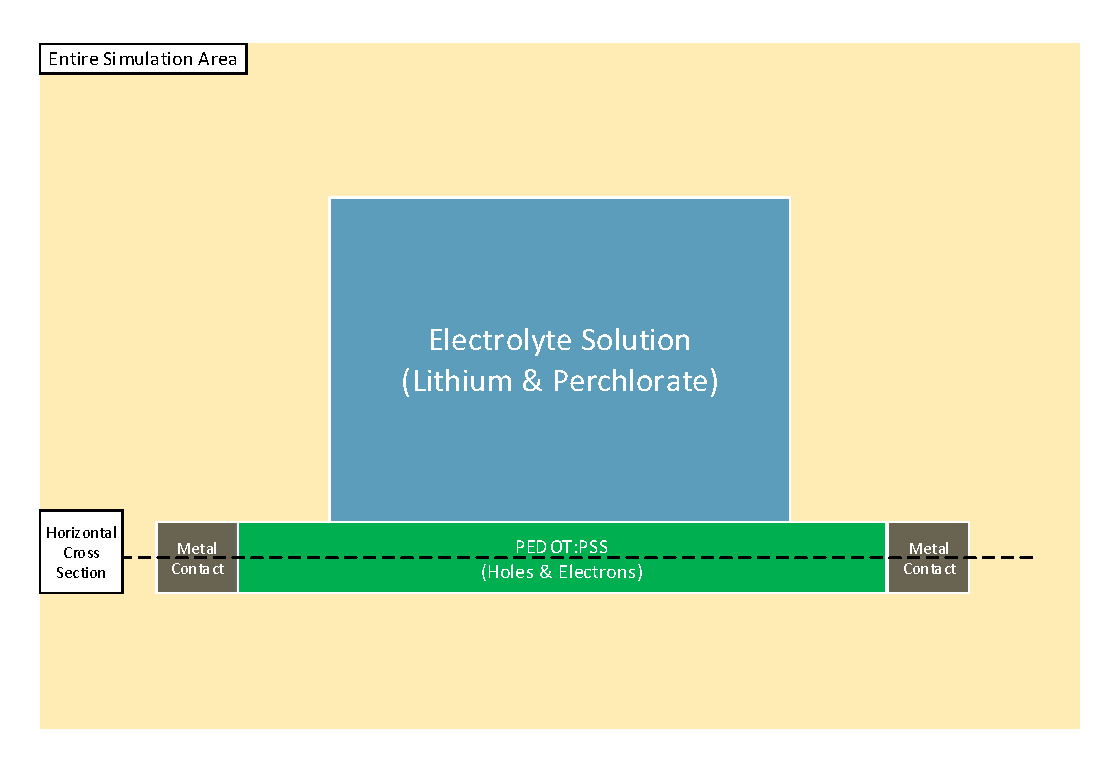
\includegraphics[scale=0.7]{Mem1}
\caption{The structure of the memristor used for simulation (not to scale)} 
\label{MemStc}
\end{figure}


The initial conditions for all the charge carriers are the same. Negative and positive charges are balanced and uniformly distributed. Perchlorate ions are not allowed to move outside the electrolyte solution so a no flow boundary condition is used around the electrolyte. Lithium ions are free to move between PEDOT:PSS and the electrolyte solution but their maximum concentration is limited inside the PEDOT:PSS. The mobility of the lithium ions has further restrictions inside PEDOT:PSS. Lithium ions have higher mobility in PEDOT:PSS under the electrolyte solution, referred as wet PEDOT:PSS, than the region without any contact with electrolyte, dry PEDOT:PSS. In fact due to this difference only a very little amount of lithium reaches the metal contacts. This decrease in the mobility was modeled by making the mobility of lithium a function of position in PEDOT:PSS. The mobility of lithium ions were assumed to be 100 times slower than the mobility of holes in the wet PEDOT:PSS and it is zero in the dry PEDOT:PSS( $\mu_{hole} \approx$ $10^{-3}$ $m^2/Vs$). 


PEDOT:PSS is a regular conductor with fixed negative charge and mobile holes. Holes can move in an out of the PEDOT:PSS through the metal contacts which preserve the charge neutrality of the initial condition throughout the simulation. The interface between PEDOT and electrolyte only allows the exchange of lithium ions. During the simulation,the movement of lithium ions changes the conductivity of the PEDOT:PSS by increasing or decreasing the amount of available holes. In the actual memristor lithium ions also change the conductivity through additional physical effects like changing the mobility of holes by modifying their hopping distance. Even though the mobility of the holes can simply be made a function of the lithium density, the shape of this function is not known. The physical details of the additional effects are beyond the scope of this thesis. 

\subsection{Boundary Conditions of the Memristor Model}

For the simulation of the memristor there are two different types of equations which require boundary and initial conditions, drift diffusion and Poisson's equation. For drift diffusion equations the boundary conditions are applied on particle and current densities. For Poisson's equation the boundary conditions are applied on the electric potential or the derivative of the electric potential.
 
\subsubsection{Drift Diffusion Equations}

For the drift diffusion problem solved in this thesis there are two different possibilities for boundary conditions on three different mobile charged particles. For metal contacts the boundary condition is enforced by keeping the net charge at zero at all times. There are two sub types of no flow boundary conditions used during simulation, a regular and a dependent no flow boundary condition. A regular no flow condition is used when the particles cannot go past a certain boundary. This is achieved by setting the particle flow at any boundary to zero (\textit{J = 0}). 

Dependent no flow boundary condition is a term that is used to describe a boundary condition which can be a function of any variable such as temperature, particle or charge density. For the lithium ions this condition is a function of lithium density and it is used not only for the boundaries but also for the points inside the PEDOT:PSS. The density limiting behavior is captured in the model by blocking the particle flow into an area if the density will go over a set limit. This can be achieved in two different ways. 

A soft limit can be set by making the particle mobility and diffusivity a function of its density. This function can be defined in such a way that it switches from a high to a low value when the particle density approaches a defined limit. This implementation is straightforward and can be used in commercial simulators but it has some drawbacks. Once the maximum particle density is reached the mobility and the diffusivity of the lithium particles are stuck at very low values. If there is an outflux of particles from that particular area then the lithium density is stuck at the limit until the mobility and the diffusivity function goes back to a value which allows more particle flow. This can introduce a considerable lag in the response of the device.  

An alternative approach is pre-calculating the particle density of a density limited node at the next time step, setting any influx to zero if the density is going to go over the limit and finally recalculating the particle densities at the next time step using the updated current densities. This mechanism sets a hard limit on the density since there is a sudden break instead of a gradual slowdown in the current flow. This density limiting mechanism is more responsive than the previous one but it requires the calculation of the next time step twice for the species that has a limit. Also a large influx of particles caused by either a big time step or a high electric field can force the algorithm to cut the current flow into a node before the density reaches its limit.

To avoid adding any unwanted lag into the system the latter method is used for the memristor simulations in this thesis. This method is implemented in the finite difference drift diffusion solver. Also a soft limit is implementend in COMSOL for comparison since it does not support the hard limit method.

Figures \ref{bc_hole}, \ref{bc_lithium} and \ref{bc_perchlorate} show the boundary conditions used for holes, lithium and perchlorate ions.

\begin{figure}[!htp]
\centering
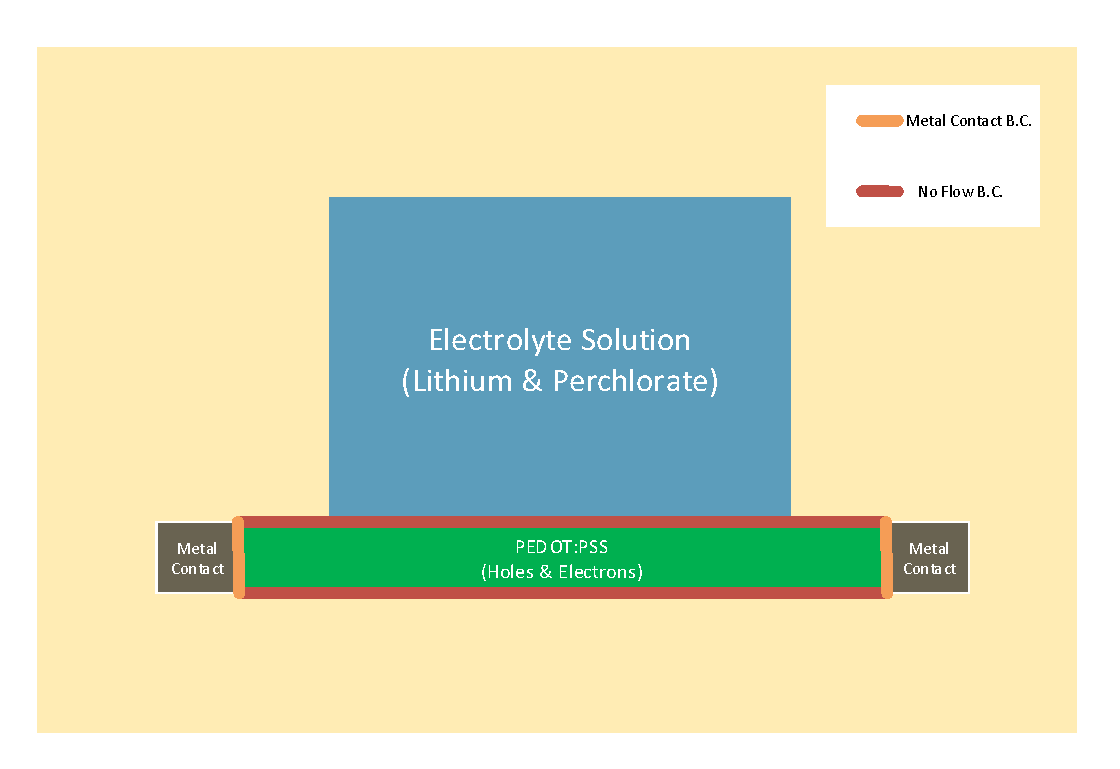
\includegraphics[scale=0.6]{bc_hole}
\caption{Boundary conditions for the holes } 
\label{bc_hole}
\end{figure}

\begin{figure}[!htp]
\centering
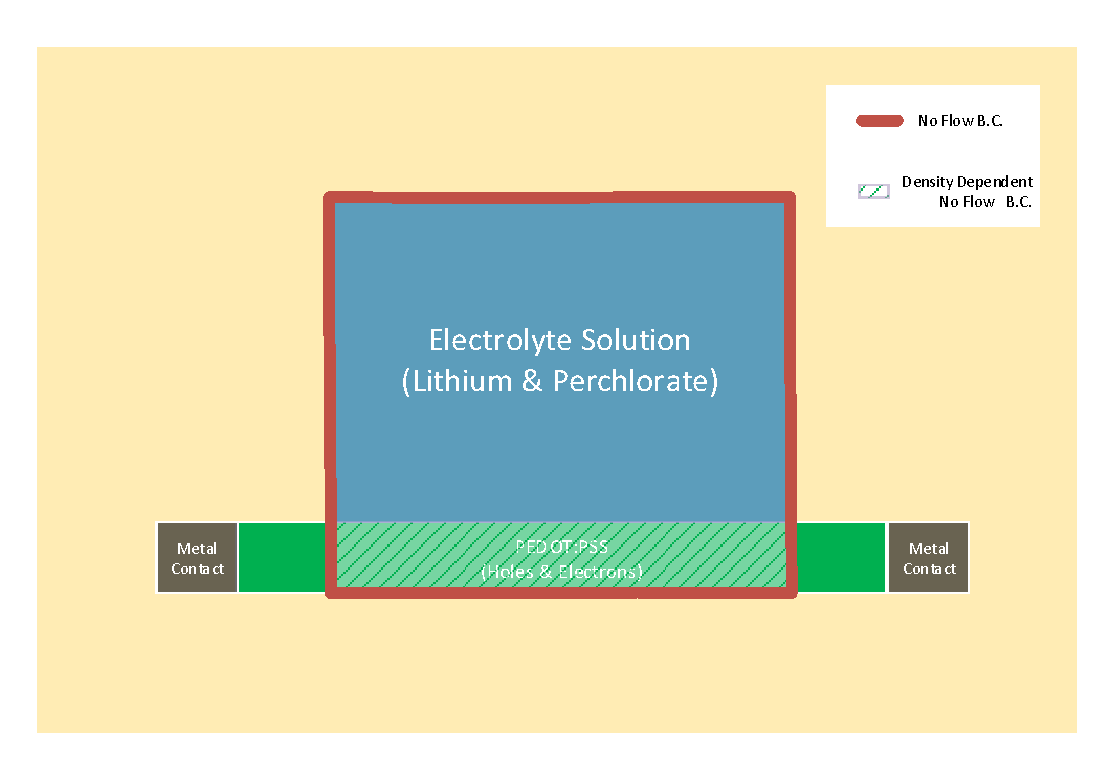
\includegraphics[scale=0.6]{bc_lithium}
\caption{Boundary conditions for the lithium ions } 
\label{bc_lithium}
\end{figure}

\begin{figure}[!htp]
\centering
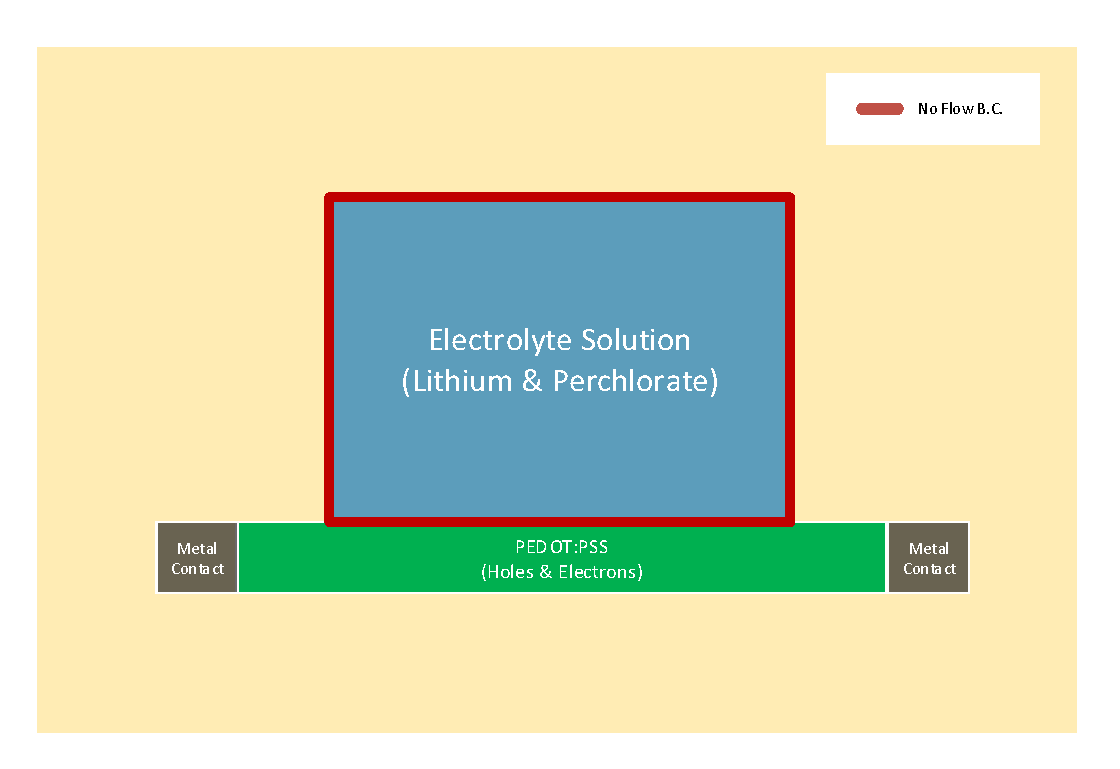
\includegraphics[scale=0.6]{bc_perchlorate}
\caption{Boundary conditions for the perchlorate ions } 
\label{bc_perchlorate}
\end{figure}




\clearpage
\subsubsection{Metal Contacts}
To simulate the metal contacts it is assumed that they hold an unlimited amount of positive and negative charges and the boundary is always charge neutral (add ref). For example for holes, electrons, positive and negative ions it is assumed that at the boundary positive charge concentration will be equal to the negative charge concentration. 

\begin{equation}
 N_{Li} + p = n + N_{ClO_{4}}
\label{chargeneutrality}
\end{equation}

In semiconductor like devices holes and electrons have to obey the mass action law.

\begin{equation}
np=n_i^2
\label{massaction}
\end{equation}

$n_i$ is the concentration at equilibrium before any ions move into the PEDOT:PSS. Solving \eqref{massaction} and \eqref{chargeneutrality} together results in the equation below:

\begin{equation}
p=\frac{1}{2}(N_{ClO_{4}} -  N_{Li} + \sqrt{(N_{ClO_{4}} -  N_{Li})^2+4n_i^2})
\label{nbound}
\end{equation}

Equation \ref{nbound} can be further simplified to equation \ref{nboundsimpl} by observing that lithium and perchlorate ions never reach the metal contact through PEDOT:PSS therefore their density will always be zero for the setup shown in (ref to 3d pic).  

\begin{equation}
p=ni
\label{nboundsimpl}
\end{equation}

During simulation, the application of the metal contact boundary condition differs from the no flow boundary which is applied implicitly. All the boundaries are simulated using a no flow condition by default but for metal contacts boundary values are set to the appropriate values at the end of every time step. The lack of charge is compensated and excess charge is taken off by the metal contact. The difference between the boundary value of the charge density and its actual value is used to calculate the derivative of the current density with respect to time. The current in and out of the device is calculated by integrating the derivative of the current density over time. 

\begin{equation}
\frac{dn}{dt}=\frac{n_{cr}-n_{ct}}{\Delta t}
\end{equation}

$n_{cr}$ is the excess carrier density and $n_{ct}$ is the equilibrium carrier density at the contact. Using these boundary conditions for holes and electrons and the following two equations it is possible to calculate incoming and outgoing currents. 

\begin{equation}
Q=An
\label{charge_charge_density}
\end{equation} 

\begin{equation}
I=\frac{dQ}{dt}
\label{current_charge}
\end{equation} 
 

Equation \ref{charge_charge_density} is an approximate relationship between charge and charge density where Q is total charge, A is the area holding that charge. Equation \ref{current_charge} is simply the general definition of current. By combining these two equations it is possible to derive a formula for calculating the current leaving or entering the device at any metal contact.

\begin{equation}
I=A \frac{dn}{dt}
\label{current_charge_density}
\end{equation}

\subsubsection{Poisson's Equation}
Discrete Poisson's equation (\ref{discrete_poisson}) is valid for almost all the nodes in the system except the boundary nodes. There are two different types of boundary conditions. The first one is Dirichlet boundary condition which forces a particular value for the potential at the boundary.

\begin{equation}
V_{i,j}=V_{b}
\label{dirichlet}
\end{equation}

Where $V_{b}$ is the value of the potential at the boundary. The other possible boundary condition is called Neumann boundary condition which states that the derivative of the potential at the boundary is zero. This gives the following equation:

\begin{equation}
\frac{\partial V}{\partial x}=\frac{V_{i+1,j}-V_{i,j}}{\Delta}=0
\label{neumannx}
\end{equation}

So for a boundary in y direction:

\begin{equation}
V_{i+1,j}=V_{i,j}
\label{neumanny}
\end{equation}

Neumann boundary condition in x direction is obtained by using the same procedure.

\begin{equation}
V_{i,j+1}=V_{i,j}
\end{equation}

Neumann boundary condition is used to let the potential float at the edge of the simulation domain and Dirichlet boundary condition is used to set applied potentials at the metal contacts. These boundary conditions are shown in figure \ref{bc_V}.

\begin{figure}[!htp]
\centering
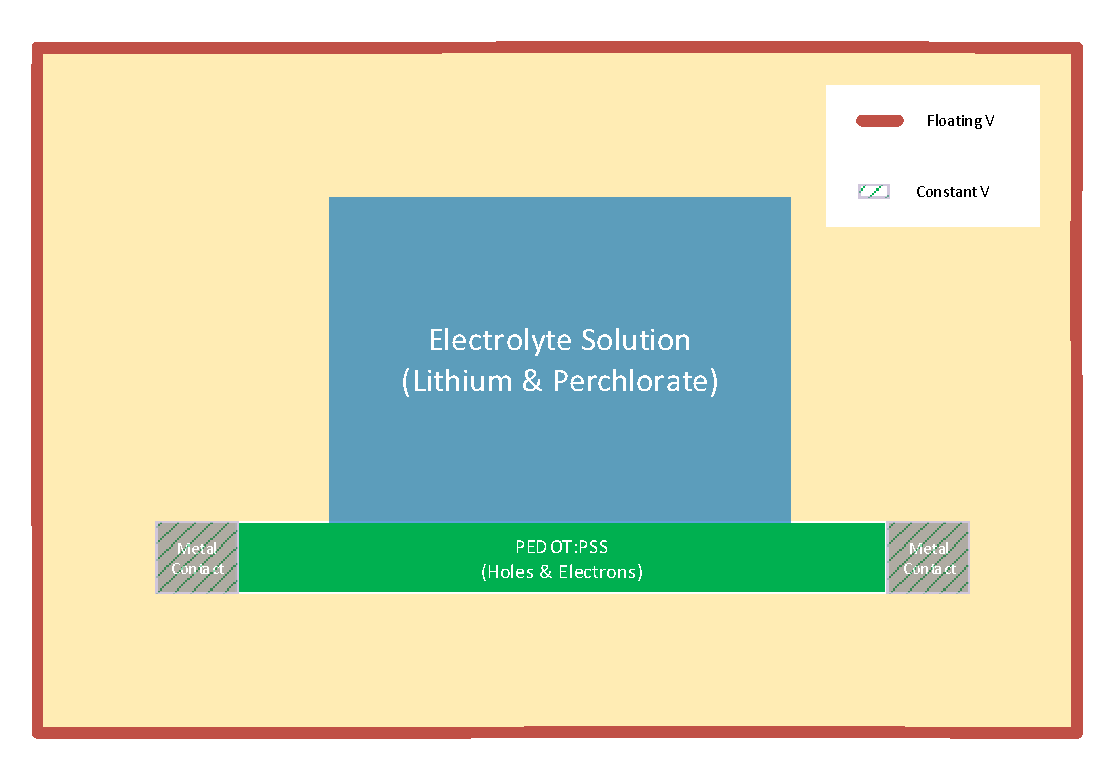
\includegraphics[scale=0.6]{bc_V}
\caption{Boundary conditions for electric potential } 
\label{bc_V}
\end{figure}

\clearpage
\section{Simulation Requirements}

It is important to analyze the computational requirements of a simulation in order to asses the feasibility of the computational scheme. In this case, it is possible to determine the spacial and the temporal requirements using the equations \ref{debye} and \ref{CFL_Drift} which describe physical and numerical limitations of the simulation. The following graph \ref{SpaceTime} shows the requirements for a memristor of the scale discussed above and a typical semiconductor device size around 1 $\mu$m. The mesh density has to be high enough in order to capture the exponential charge accumulation for charge shielding so the minimum step size was set to be 5 times smaller than the Debye length. The plots \ref{SpaceTime}.a and \ref{SpaceTime}.c show the amount of points required to simulate a semiconductor and a memristor based on minimum step size. It is important to note that these values are for 1-D simulation and they can be converted to 2-D and 3-D by taking the square or the cube of the values in \textit{y} axis respectively. Plots \ref{SpaceTime}.b and \ref{SpaceTime}.d are created using CFL conditions for drift and diffusion and dielectric relaxation time. A typical simulation time is estimated using the mobility and the electric field. Based on the estimated simulation time the number of time steps are calculated using the minimum time step obtained from CFL conditions and dielectric relaxation time.

It can be seen from graphs \ref{SpaceTime}.a and \ref{SpaceTime}.c that memristor simulations require much higher mesh densities compared to a typical semiconductor simulation such as 1 $\mu$m long PN diode. This is due to the larger size and higher charge density of the memristor. Plots \ref{SpaceTime}.a and \ref{SpaceTime}.b show that a memristor with $10^{26}$ $m^{-3}$ charge density requires close to $10^9$ points and $10^{14}$ time steps to simulate in 1-D. These requirements make the simulation of the memristor extremely challenging. In order to investigate and find possible solutions to this issue, first a memristor with low charge density ($\approx 10^{15}$) is simulated in order to ensure that the simulation functions as designed. Then memristors with different charge densities are simulated and compared to each other to asses whether the behavior at low charge densities will be comparable to the behavior at high charge densities.

\begin{landscape}
\begin{figure}[htp]
\centering
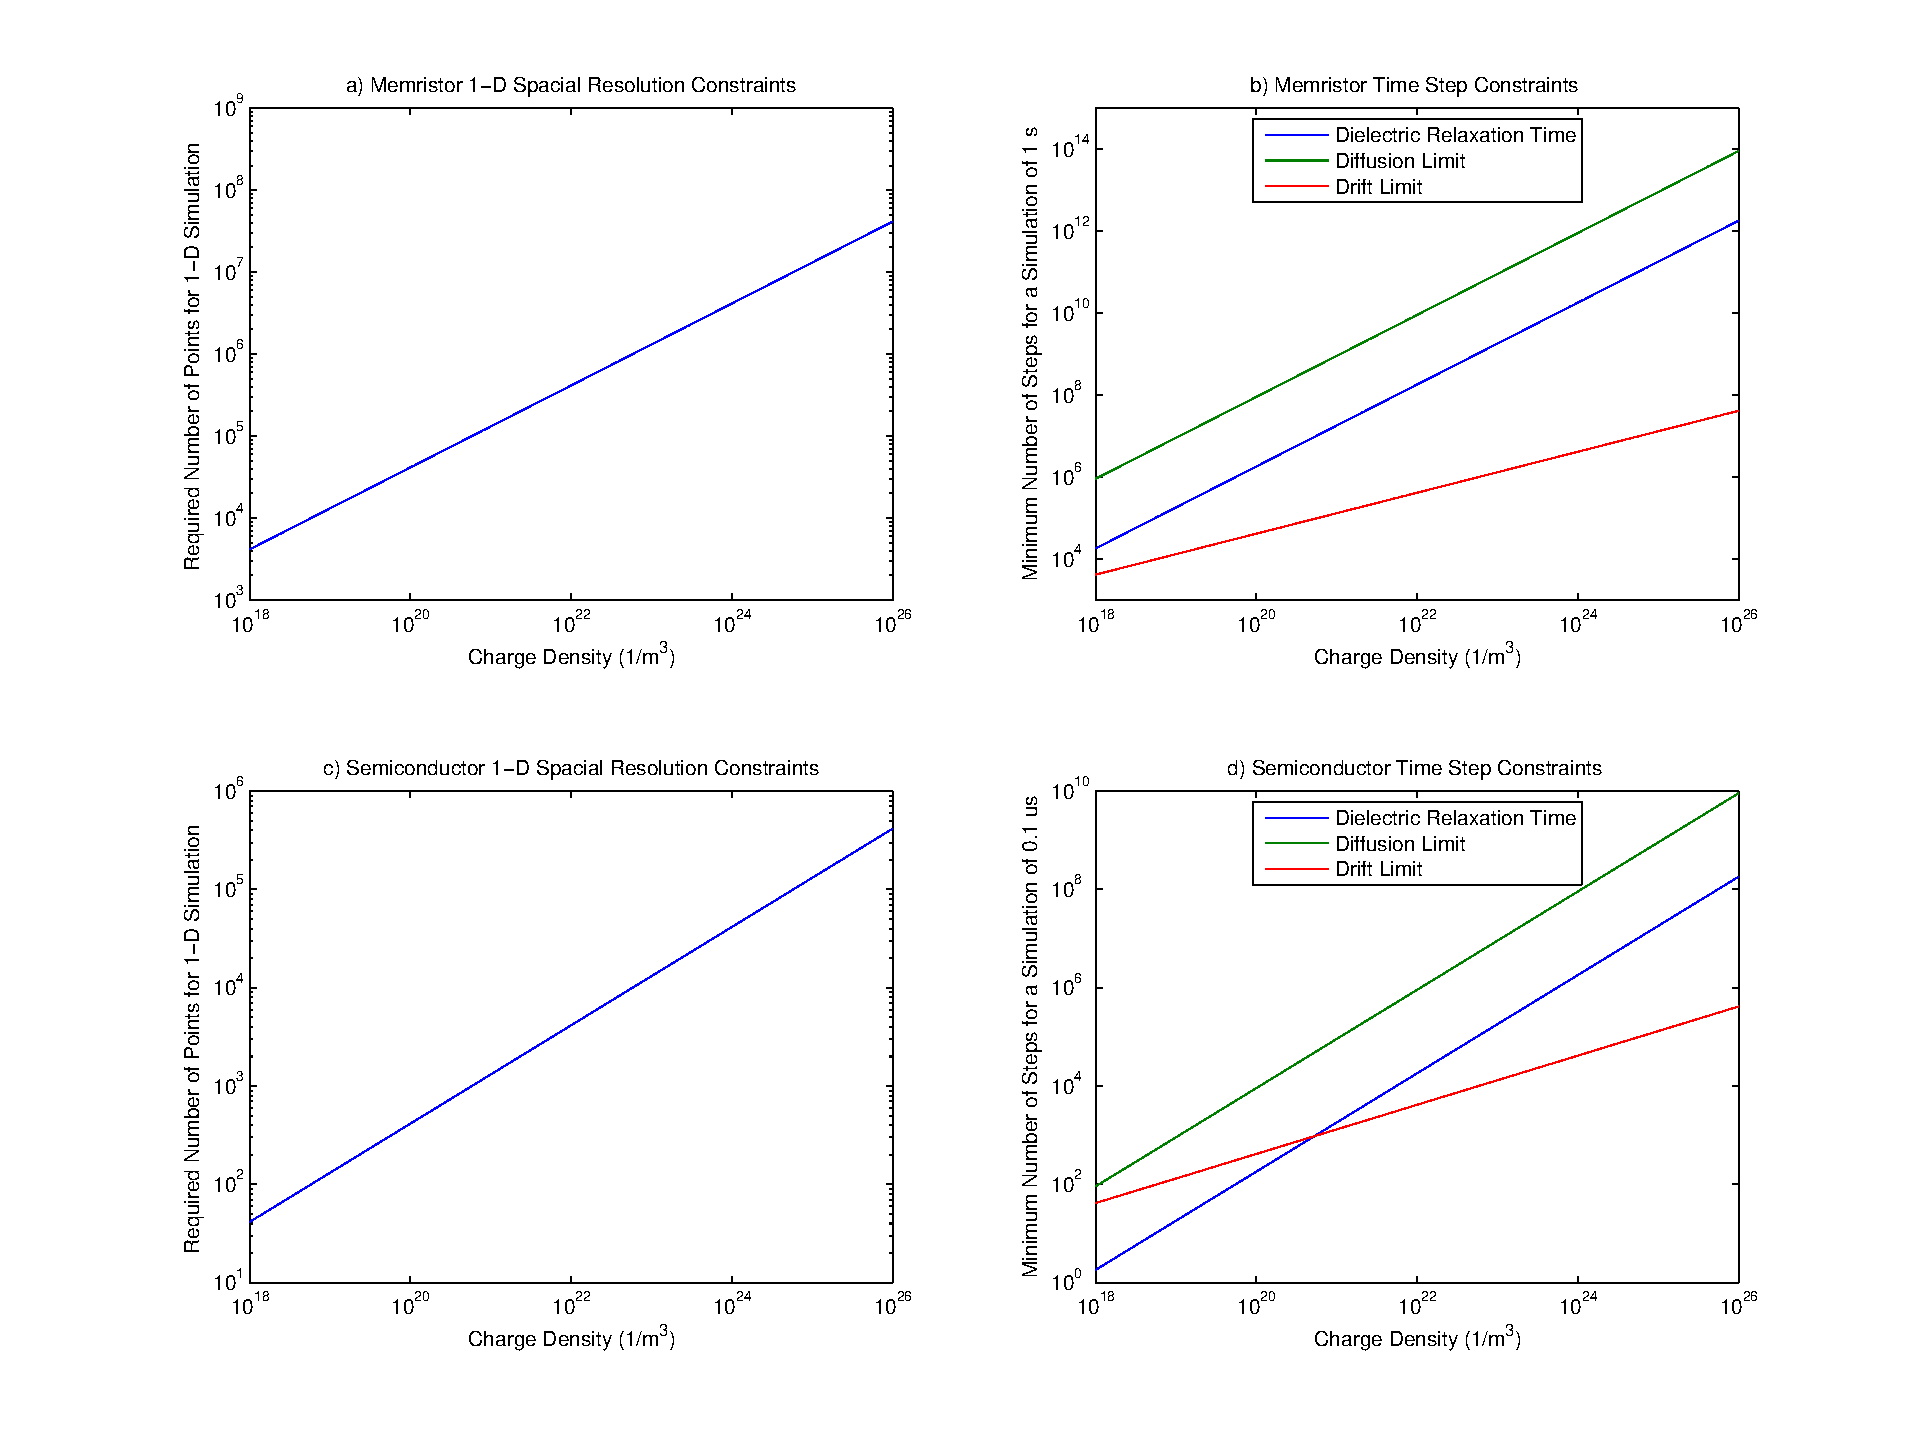
\includegraphics[scale=0.60]{SpaceTime}
\caption{Spatial and temporal requirements for simulation} 
\label{SpaceTime}
\end{figure}
\end{landscape}

\end{doublespace}
